\subsubsection{User Settings Page Specifications}
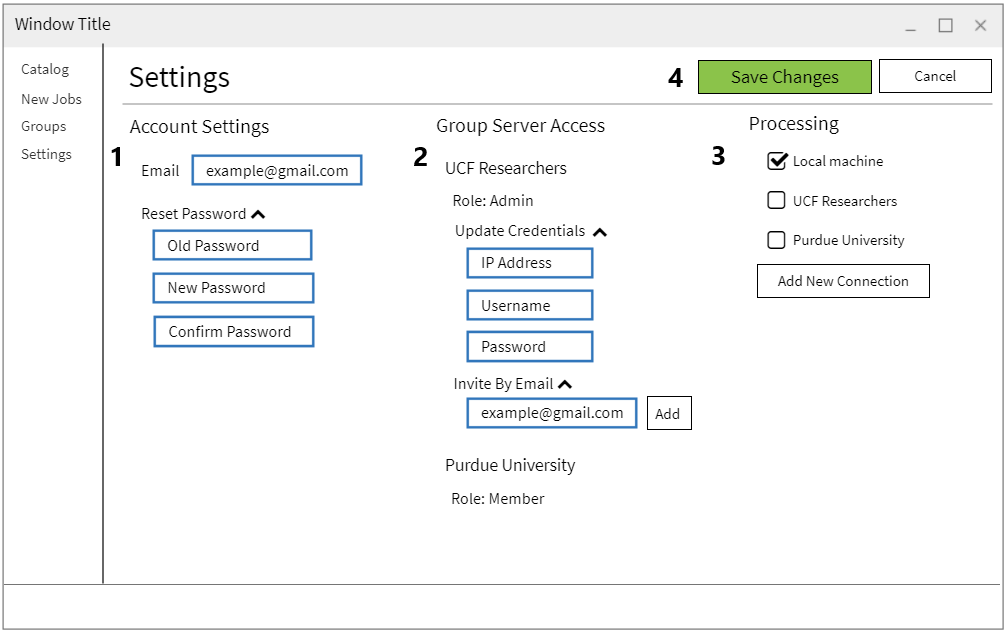
\includegraphics[width=\textwidth]{SettingsPage}\\
The settings page is where the user can change their account information, update shared server access, and choose their processing location. The settings page is important for the user and thus should be explained in as much detail as possible. The core functionality of the settings page includes:\\
\begin{enumerate}
    \item \textbf{Account Settings}\\ Here the user can update their account username and password. This is a simple section, but highly important for users.
    \item \textbf{Group Server Access}\\ This section includes the servers that the user has access to and the credentials for them. For groups that a user is an admin, they can update the IP address for that server as well as the login credentials for public access. They can also invite others to access this public directory. For groups where the user is just a member, they can just choose it as a processing location where applicable.
    \item \textbf{Processing Location}\\ The processing section is where the user can define where they would like to run the jobs. These locations are servers they have access to where sound files are stored. These locations also have the server application running on them. This is useful for the user because they can have multiple locations for file storage \textit{and} processing.
    \item \textbf{Saving Changes}\\ When selected, the Save Changes button will save any user settings and processing options for the user.
\end{enumerate}